\chapter{Технологическая часть}

В данной части представляется выбор средств реализации, описывается организация классов в программе и представляется интерфейс.

\section{Средства реализации}

В качестве языка программирования для реализации данной курсовой работы был выбран $C\#$ по следующим причинам:
\begin{itemize}[label=--]
	\item в стандартной библиотеке $C\#$ присутствуют необходимые структуры и классы, выбранные по результатам проектирования;
	\item поддержка объектно-ориентированного программирования;
	\item поддержка асинхронного программирования.
\end{itemize}

\section{Структура программы}

Разработанная программа состоит из следующих классов:
\begin{enumerate}
	\item управляющий классы:
	\begin{itemize}[label=--]
		\item \textit{Program} -- точка входа в программу.
	\end{itemize}
	\begin{figure}[h] 
		\centering
		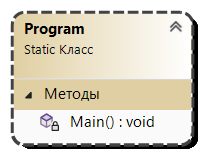
\includegraphics[width=0.2\textwidth]{images/main-class.png}
		\caption{Управляющий класс} 
		\label{fig:main-class} 
	\end{figure}
	\item классы интерфейса:
	\begin{itemize}[label=--]
		\item \textit{Form1} -- главное окно программы;
		\item \textit{DialogEdit} -- окно редактирования модели;
		\item \textit{ErrorMessage} -- окно, содержащее сообщение об ошибке.
	\end{itemize}
	\clearpage
	\begin{figure}[h] 
		\centering
		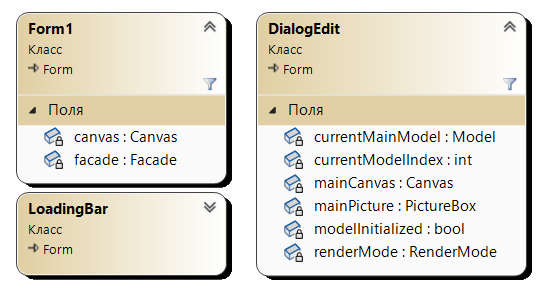
\includegraphics[width=0.5\textwidth]{images/interface-class.png}
		\caption{Классы интерфейса} 
		\label{fig:interface-class} 
	\end{figure}
	\item классы инкапсуляции действий:
	\begin{itemize}[label=--]
		\item \textit{Command} -- базовый класс команды для выполнения;
		\item \textit{SceneCommand} -- базовый класс команды для обработки сцены;
		\item \textit{CameraCommand} -- базовый класс команды для обработки камеры;
		\item \textit{DrawsCommand} -- базовый класс команды для обработки экрана;
		\item \textit{TransformationCommand} -- базовый класс команды для преобразований объектов;
		\item \textit{FormCommand} -- базовый класс команды для обработки интерфейса.
	\end{itemize}
	\begin{figure}[h] 
		\centering
		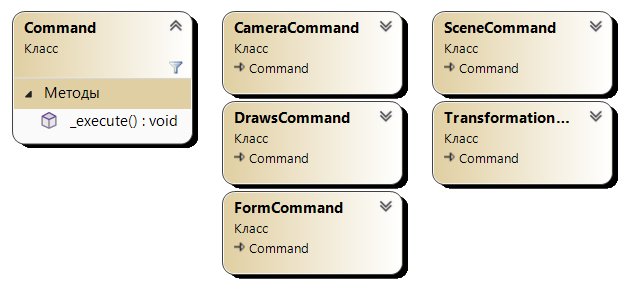
\includegraphics[width=0.6\textwidth]{images/commands-class.png}
		\caption{Классы инкапсуляции действий} 
		\label{fig:commands-class} 
	\end{figure}
	\item классы обработки команд:
	\begin{itemize}[label=--]
		\item \textit{Facade} -- единый интерфейс для обработки команд;
		\item \textit{SceneManager} -- обработчик команд, работающих со сценой;
		\item \textit{DrawManager} -- обработчик команд, работающих с экраном;
		\item \textit{TransformationManager} -- обработчик команд, преобразовывающих объекты;
		\item \textit{FormManager} -- обработчик команд, работающих с интерфейсом.
	\end{itemize}
	\begin{figure}[h] 
		\centering
		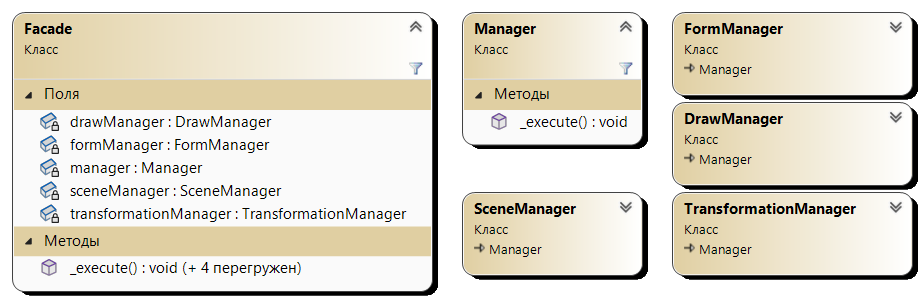
\includegraphics[width=0.8\textwidth]{images/commandsprocessors-class.png}
		\caption{Классы обработки команд} 
		\label{fig:commandsprocessors-class} 
	\end{figure}
	\item классы взаимодействия со сценой:
	\begin{itemize}[label=--]
		\item \textit{Canvas} -- менеджер изображения на экране;
		\item \textit{Scene} -- менеджер трехмерной сцены;
		\item \textit{ViewingSystem} -- менеджер просмотра сцены.
	\end{itemize}
	\begin{figure}[h] 
		\centering
		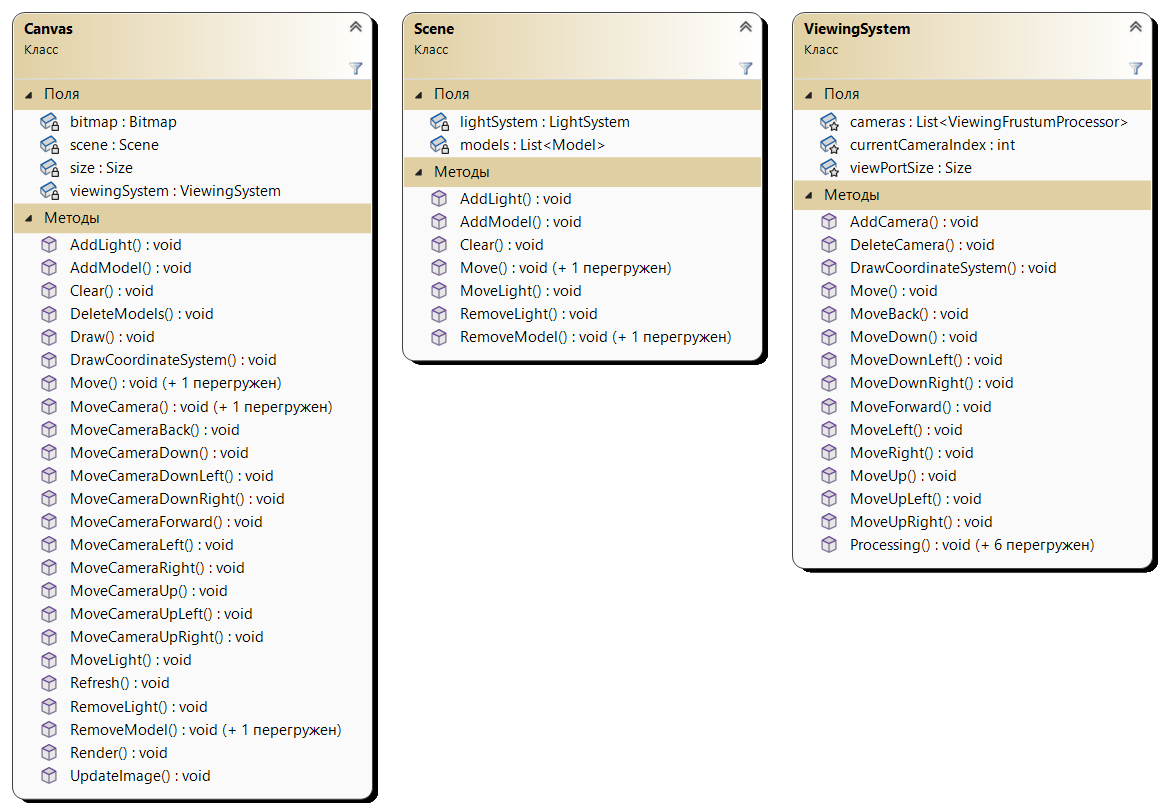
\includegraphics[width=0.8\textwidth]{images/canvas-class.png}
		\caption{Классы взаимодействия со сценой} 
		\label{fig:canvas-class} 
	\end{figure}
	\item классы представления света:
	\begin{itemize}[label=--]
		\item \textit{LightSystem} -- менеджер источников света;
		\item \textit{Light} -- источник света.
	\end{itemize}
	\clearpage
	\begin{figure}[h] 
		\centering
		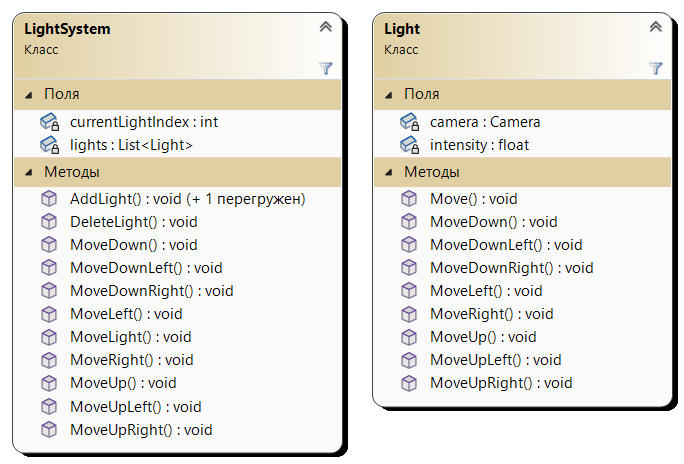
\includegraphics[width=0.6\textwidth]{images/light-class.png}
		\caption{Классы представления света} 
		\label{fig:light-class} 
	\end{figure}
	\item классы представления моделей:
	\begin{itemize}[label=--]
		\item \textit{Model} -- базовый класс многогранной модели;
		\item \textit{Cube} -- куб;
		\item \textit{DirectPrism} -- прямая призма;
		\item \textit{Pyramid} -- триугольная пирамида.
	\end{itemize}
	\begin{figure}[h] 
		\centering
		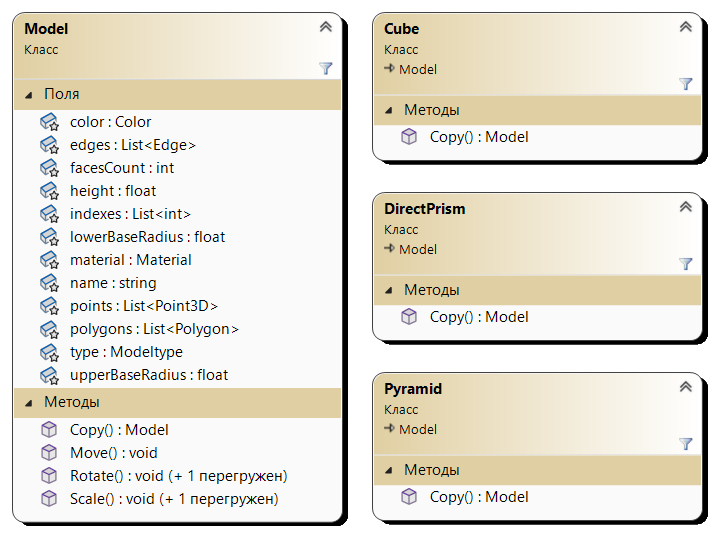
\includegraphics[width=0.6\textwidth]{images/model-class.png}
		\caption{Классы представления моделей} 
		\label{fig:model-class} 
	\end{figure}
	\item классы представления камеры:
	\begin{itemize}[label=--]
		\item \textit{Camera} -- камера;
		\item \textit{ViewingFrustum} -- камера, учитывающая видимое пространство и визуализирующая сцену с использованием перспективных преобразований;
		\item \textit{ViewingFrustumZBuffer} -- камера, учитывающая видимое пространство, визуализирующая сцену с использованием перспективных преобразований и удалением невидимых линий и поверхностей;
		\item \textit{ViewingFrustumParallelZBuffer} -- камера \textit{ViewingFrustumZBuffer}, реализованная с использованием параллельных потоков;
		\item \textit{ViewingFrustumPhongShading} -- камера, учитывающая видимое пространство, визуализирующая сцену с использованием перспективных преобразований, удалением невидимых линий и поверхностей и расчетом освещенности объектов;
		\item \textit{ViewingFrustumParallelPhongShading} -- камера \newline \textit{ViewingFrustumPhongShading}, реализованная с использованием параллельных потоков;
		\item \textit{ViewingFrustumShadows} -- камера, учитывающая видимое пространство, визуализирующая сцену с использованием перспективных преобразований, удалением невидимых линий и поверхностей, расчетом освещенности объектов и возникающих теней;
		\item \textit{ViewingFrustumParallelShadows} -- камера \textit{ViewingFrustumShadows}, реализованная с использованием параллельных потоков;
		\item \textit{ViewingFrustumProcessor} -- камера с многорежимной визуализацией сцены.
	\end{itemize}
	\clearpage
	\begin{figure}[h] 
		\centering
		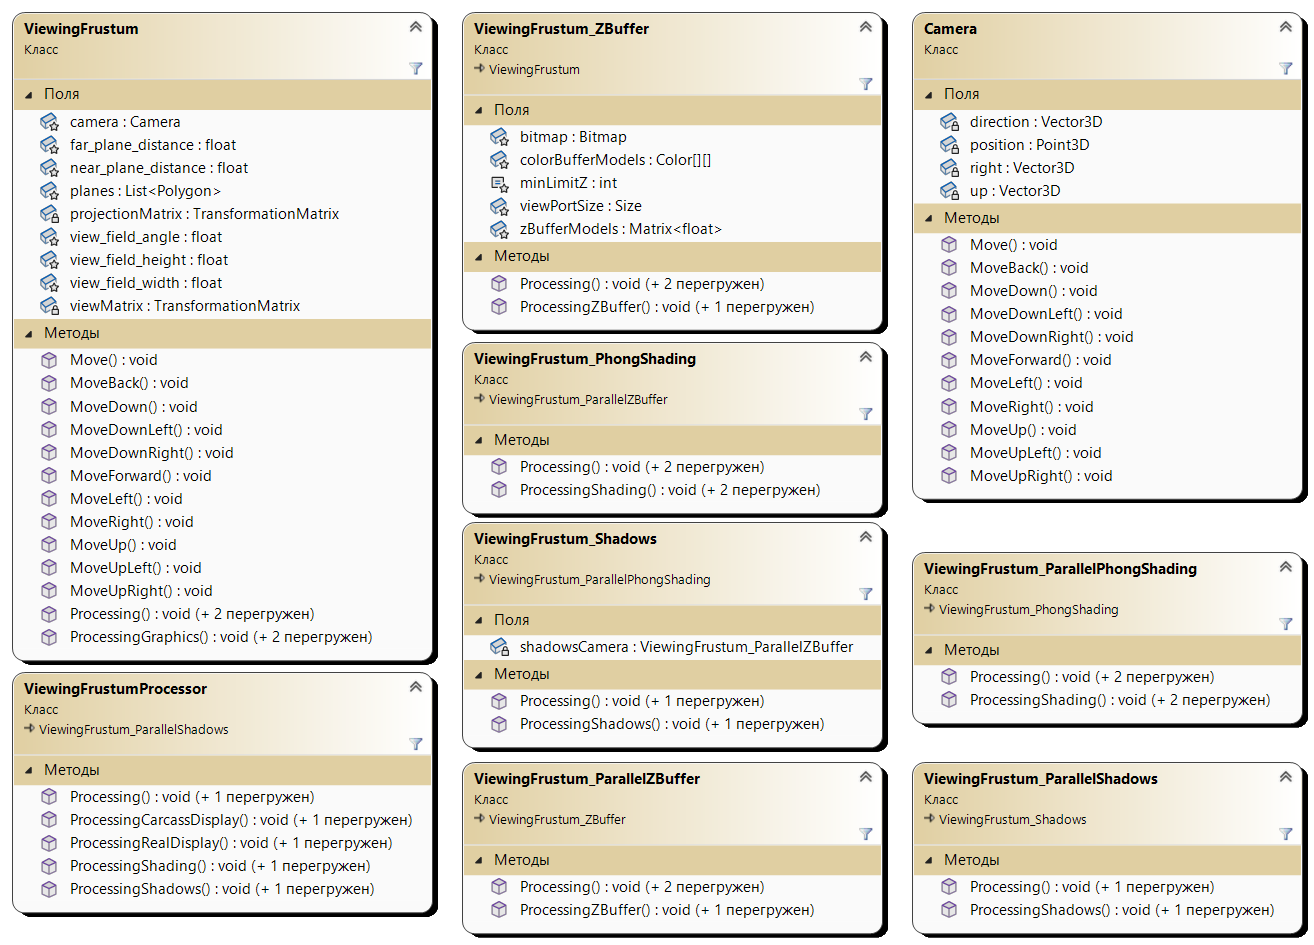
\includegraphics[width=1\textwidth]{images/camera-class.png}
		\caption{Классы представления камеры} 
		\label{fig:camera-class} 
	\end{figure}
	\item классы афинных преобразований:
	\begin{itemize}[label=--]
		\item \textit{Transformation} -- базовый класс афинного преобразования;
		\item \textit{Move} -- перемещение;
		\item \textit{Rotate} -- поворот;
		\item \textit{Scale} -- масштабирование.
	\end{itemize}
	\begin{figure}[h] 
		\centering
		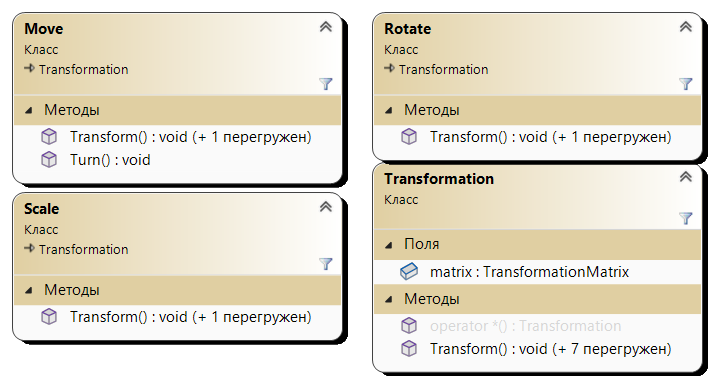
\includegraphics[width=0.532\textwidth]{images/transformation-class.png}
		\caption{Классы аффинных преобразований} 
		\label{fig:transformation-class} 
	\end{figure}
	\item математические классы:
	\begin{itemize}[label=--]
		\item \textit{Matrix} -- матрица;
		\item \textit{TransformationMatrix} -- матрица афинного преобразования;
		\item \textit{Vector3D} -- трехмерный вектор.
	\end{itemize}
	\begin{figure}[h] 
		\centering
		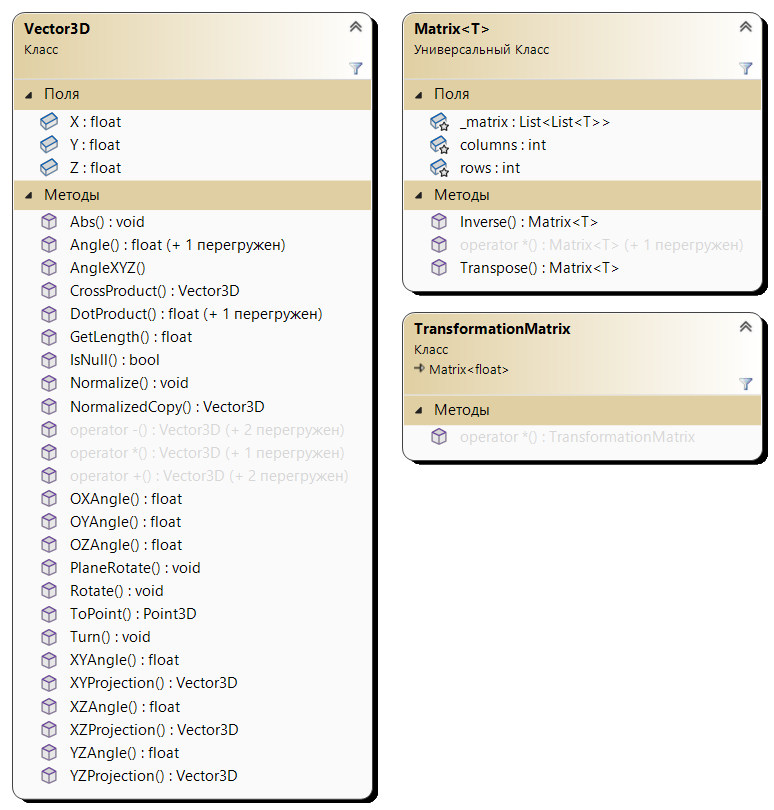
\includegraphics[width=0.7\textwidth]{images/math-class.png}
		\caption{Математические классы} 
		\label{fig:math-class} 
	\end{figure}
\end{enumerate}


\section{Интерфейс программы}

...

\section*{Вывод}

<что делали и получили в результате>

\clearpage
